\documentclass[11pt,a4paper]{article}

% ---------------------------------------------------------------------------
% Objective 2 report: grounding the kiosk assistant with retrieval and a refusal fallback
% Compile with:  pdflatex objective2_report.tex  (run twice for references)
% Figures are expected in ./figs/ (produced by make_figs.py).
% ---------------------------------------------------------------------------

\usepackage[margin=2.4cm]{geometry}
\usepackage[T1]{fontenc}
\usepackage{mathpazo}
\usepackage{microtype}
\usepackage{graphicx}
\usepackage{booktabs}
\usepackage{tabularx}
\usepackage{xltabular}
\usepackage{array}
\usepackage{multirow}
\usepackage{xcolor}
\usepackage{enumitem}
\usepackage{amsmath}
\usepackage{caption}
\usepackage{float}
\usepackage{tikz}
\usetikzlibrary{arrows.meta,positioning,shapes.geometric,fit,calc}
\usepackage[hidelinks]{hyperref}

\definecolor{ink}{HTML}{0B0B0B}
\definecolor{ink2}{HTML}{52514E}
\definecolor{qblue}{HTML}{2A78D6}
\definecolor{qorange}{HTML}{EB6834}
\definecolor{qaqua}{HTML}{1BAF7A}
\definecolor{qred}{HTML}{C9302C}
\definecolor{boxfill}{HTML}{F3F7FD}
\definecolor{metfill}{HTML}{E5F4E4}
\definecolor{missfill}{HTML}{FBEBEB}

\captionsetup{font=small,labelfont=bf}
\setlist{itemsep=2pt,topsep=4pt}
\renewcommand{\arraystretch}{1.18}
\newcolumntype{L}{>{\raggedright\arraybackslash}X}
\newcommand{\met}{\textcolor{qaqua}{\textbf{met}}}
\newcommand{\missed}{\textcolor{qred}{\textbf{missed}}}

% Placeholder: replace before submission
\newcommand{\placeholder}[1]{\textcolor{red}{[#1]}}
\newcommand{\reportdate}{23 September 2026}

\title{\textbf{Grounding a Small-Model Retail Kiosk Assistant\\in Store Knowledge}\\[4pt]
\large Objective 2: Grounded Retrieval with a Refusal Fallback}
\author{Anany Dev Choudhary\\\small Roll No.\ 228070135\\\small Department of Electrical Engineering\\\small Indian
Institute of Technology Kanpur}
\date{\reportdate}

\begin{document}
\maketitle

\begin{abstract}
\noindent
Objective~1 selected two small language models for an offline in-store kiosk: Qwen3.5-4B (4-bit) for kiosks with an
integrated GPU and Qwen3.5-2B (8-bit) for CPU-only kiosks. Both could call catalogue tools, but neither had access to
the store's knowledge: its policies, services, offers, store hours, product descriptions and watch-care advice. This
report adds that knowledge through retrieval, and adds a fallback that refuses when nothing relevant is found. The work
scaled a fictional watch catalogue to 1,518 products and built an 812-chunk knowledge corpus from it. It wrote a
500-question retrieval evaluation set with gold answers and a fixed dev/test split, and benchmarked 21 retrieval
configurations on CPU. The fallback threshold was calibrated on dev questions only. The retriever was then integrated
into the assistant and the system evaluated end to end on 373 test questions and the 234 tool cases of Objective~1,
under five conditions per model. Every decision rule was written down before the run it governed, and every target is
reported as met or missed.
The chosen retriever, hybrid BM25 + bge-small with a MiniLM cross-encoder, finds a correct chunk in the top five for
92\% of test questions and adds about 0.9\,GB of memory. With retrieval, \textbf{Qwen3.5-4B answers 77.9\% of answerable
test questions correctly, against 50.0\% without it}, within 4.1 points of being handed the correct text directly. It
also refuses only 5.4\% of answerable questions, and replies faster than without retrieval. Retrieval cut judged
hallucination on unanswerable questions from 30\% to 19\% (4B) and from 40\% to 23\% (2B). The 5\% hallucination
target, the 300\,ms retrieval-latency target and the memory target are all missed. Retrieval also lowered the pass rate
on Objective~1's tool cases (4B: 78\% to 72\%; 2B: 69\% to 56\%). The 2B model misses most targets. A failure
analysis traces the remaining hallucinations to five model behaviours, all candidates for the prompt and tool-design
work of Objective~3.
\end{abstract}

\tableofcontents
\vspace{6pt}
\hrule

% ===========================================================================
\section{Introduction}
% ===========================================================================

\subsection{Where Objective 1 left the assistant}
Objective~1 built the kiosk assistant's ``talking'' and ``acting'' layers. A small language model runs the
conversation in English or Hinglish (Hindi--English code-mixing in Roman script). It calls seven tools: search the
catalogue, get product details, compare products, check stock, find alternatives, get offers, and call a staff member.
Two configurations were selected, one per hardware tier:
\begin{itemize}
  \item \textbf{Tier~B} (integrated GPU, $\le$10\,GB): \textbf{Qwen3.5-4B, Q4\_K\_M}, which passed 81\% of 292 test cases;
  \item \textbf{Tier~A} (CPU only, 4 threads, $\le$5\,GB): \textbf{Qwen3.5-2B, Q8\_0}, which passed 74\%.
\end{itemize}

The tools only answer questions about products in the catalogue database. A real customer also asks:
\begin{itemize}
  \item \emph{store questions}: ``When do you close?'', ``Do you deliver?'', ``Can I pay part in cash?'';
  \item \emph{policy questions}: ``Can my wife claim the warranty on a watch I bought her?'';
  \item \emph{watch-care and terminology questions}: ``What is an open-heart dial?'', ``Can I wear it in the sauna?'';
  \item \emph{offer questions}: ``What's the biggest festive discount?'';
  \item \emph{descriptive questions}: ``I want a men's formal quartz watch with a blue dial and a leather strap'';
  \item \emph{questions nothing answers}: products not sold, policies that don't exist, off-topic requests.
\end{itemize}
In Objective~1 the answers to the first kinds were pasted into the prompt by hand for the few cases that needed them.
A deployed kiosk cannot do that. A model asked such a question with nothing to read from must either refuse or invent,
and small models tend to invent.

\subsection{Objective 2}
\textbf{Objective~2} is to ground the assistant in the store's knowledge:
\begin{enumerate}
  \item build a searchable corpus of the store's knowledge;
  \item choose a retriever that runs on the kiosk's CPU next to the language model;
  \item put a \emph{refusal fallback} in front of the model, so a question that matches nothing gets an honest
        ``I don't have that information'' and an offer to call staff;
  \item integrate both into the assistant and measure the whole system end to end, against targets fixed in advance.
\end{enumerate}
This is the ``retrieval knows'' layer of the architecture adopted in Objective~1, which published on-device kiosk
designs share: the model talks, tools act, retrieval knows, and a fallback refuses~\cite{rag}.

\subsection{Contributions}
\begin{itemize}
  \item A scaled, seeded mock catalogue (1,518 SKUs) and an 812-chunk knowledge corpus, both reproducible from a seed.
  \item A 500-question retrieval evaluation set with gold chunks, checked facts, and deliberate near misses, unanswerable
        and Hinglish questions, split into dev and test before any retriever ran.
  \item A CPU benchmark of 21 retrieval configurations and 18 latency variants under fixed decision rules.
  \item A calibrated refusal fallback, and a measured fix for its bias against Hinglish questions.
  \item An integrated assistant with four retrieval conditions and three fallback modes, logged per stage.
  \item An end-to-end evaluation of both selected models on 607 test cases, with blind judging and a human check.
\end{itemize}

\subsection{Structure of this report}
Section~\ref{sec:criteria} sets out the success criteria. Section~\ref{sec:system} describes the system and
Section~\ref{sec:method} the method, step by step. Section~\ref{sec:results} gives the results.
Section~\ref{sec:decisions} records every decision and its reasoning. Section~\ref{sec:limits} lists the limitations
and Section~\ref{sec:next} the next steps.

% ===========================================================================
\section{Success criteria}\label{sec:criteria}
% ===========================================================================

The targets in Table~\ref{tab:criteria} were agreed before the first retrieval run and judged only on the test split.
As in Objective~1, a target that is missed is reported as missed and not moved.

No published standard exists for retrieval quality or speed on a kiosk catalogue, so the retrieval targets (Recall@5,
MRR, latency, memory) are this project's own bars. They were set so that retrieval is unlikely to be the weakest link:
a retriever that finds the right text nine times in ten leaves most errors to the model. Two rows were added after a
literature check, before any run:
\begin{itemize}
  \item \textbf{Near-miss hallucination.} Evaluations of retrieval-augmented small models report that misleading
        context, such as a similar but different product, makes them answer instead of abstaining. The test set
        therefore contains near misses on purpose, and they are scored separately.
  \item \textbf{Unsupported details.} Public hallucination leaderboards measure how often a model adds claims not in the
        text it was given. They report about 6\% for current 4B-class models even with the right text in
        hand~\cite{vectara}.
\end{itemize}

\begin{table}[H]
\centering
\small
\begin{tabularx}{\textwidth}{L l L}
\toprule
Criterion & Target & Measured on \\
\midrule
Recall@5 on answerable questions & $\ge$ 90\% & Retrieval test split, retriever alone \\
Mean reciprocal rank (MRR@10) & $\ge$ 0.75 & Retrieval test split, retriever alone \\
Hallucination on unanswerable questions, with the fallback & $\le$ 5\% (also reported without it) & Unanswerable test
questions, end to end \\
Hallucination on near-miss questions, with the fallback & $\le$ 5\%, reported separately & Near-miss test questions,
end to end \\
False refusals on answerable questions & $\le$ 10\% & Answerable test questions, end to end \\
Answers with retrieved text against the gold text & Within 5 points (paired) & Both selected models \\
Unsupported details in answers & $\le$ 5\% of answers & Answerable test questions, both models \\
Retrieval latency, Tier~A & p50 $\le$ 300\,ms on CPU & Measured in place \\
Added memory & $\le$ 0.8\,GB, so Tier~A stays under 5\,GB & Peak, model plus retriever \\
No regression on tool cases & Not significantly below no retrieval & The 234 v1.1 test tool cases \\
\bottomrule
\end{tabularx}
\caption{Success criteria, fixed before the first retrieval run.}
\label{tab:criteria}
\end{table}

% ===========================================================================
\section{System overview}\label{sec:system}
% ===========================================================================

Figure~\ref{fig:arch} shows the assistant as deployed at the end of this objective. Every customer message is
searched against the knowledge corpus before the model sees it. The best chunks are attached to the message only when
the retriever is confident; otherwise the message reaches the model unchanged, and the model can still use its tools
or decline. The model, the tools and the prompt are those selected in Objective~1. One rule is added to the prompt
(Appendix~\ref{app:prompt}).

\begin{figure}[H]
\centering
\resizebox{\textwidth}{!}{%
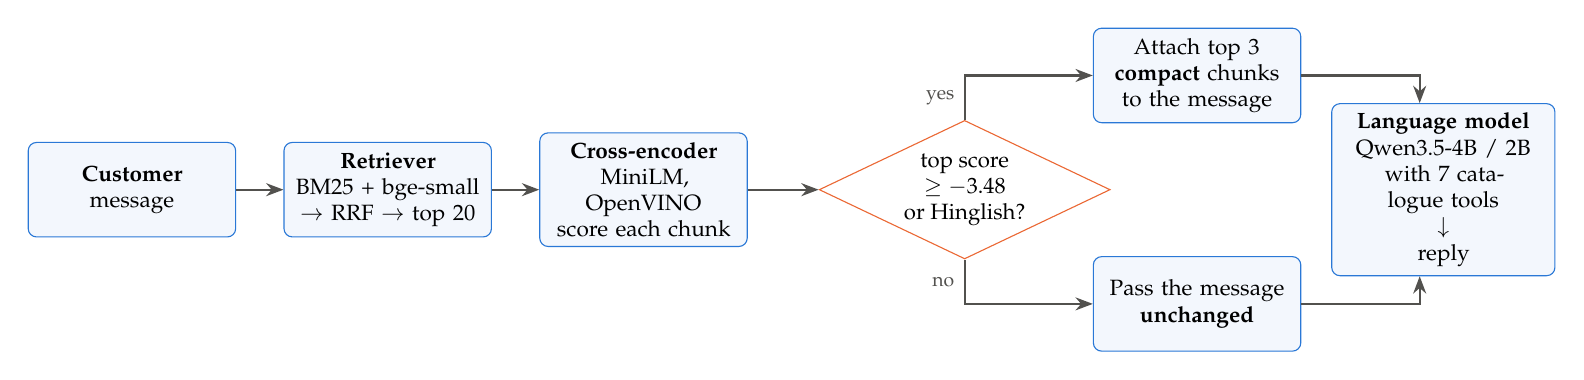
\begin{tikzpicture}[
  node distance=5mm and 6mm,
  box/.style={draw=qblue, fill=boxfill, rounded corners=3pt, align=center, font=\footnotesize, minimum height=12mm,
              text width=24mm},
  gate/.style={draw=qorange, fill=white, diamond, aspect=2.1, align=center, font=\footnotesize, inner sep=1pt},
  arr/.style={-{Stealth[length=2.2mm]}, thick, ink2}]
\node[box] (msg) {\textbf{Customer}\\message};
\node[box, right=of msg] (ret) {\textbf{Retriever}\\BM25 + bge-small\\$\rightarrow$ RRF $\rightarrow$ top 20};
\node[box, right=of ret] (rr) {\textbf{Cross-encoder}\\MiniLM, OpenVINO\\score each chunk};
\node[gate, right=9mm of rr] (g) {top score\\$\ge -3.48$\\or Hinglish?};
\node[box, above right=4mm and 7mm of g] (yes) {Attach top 3\\\textbf{compact} chunks\\to the message};
\node[box, below right=4mm and 7mm of g] (no) {Pass the message\\\textbf{unchanged}};
\node[box, right=28mm of g, text width=26mm, minimum height=20mm] (llm) {\textbf{Language model}\\Qwen3.5-4B / 2B\\with 7 catalogue
tools\\$\downarrow$\\reply};
\draw[arr] (msg) -- (ret);
\draw[arr] (ret) -- (rr);
\draw[arr] (rr) -- (g);
\draw[arr] (g.north) |- node[pos=0.25, left, font=\scriptsize] {yes} (yes.west);
\draw[arr] (g.south) |- node[pos=0.25, left, font=\scriptsize] {no} (no.west);
\draw[arr] (yes.east) -| ($(llm.north)+(-0.3,0)$);
\draw[arr] (no.east) -| ($(llm.south)+(-0.3,0)$);
\end{tikzpicture}}
\caption{The deployed assistant. Retrieval takes about 0.5\,s on four CPU threads. ``Compact'' chunks are product cards
without their marketing description. A re-fetch of a product already shown returns a short pointer instead of the full
record (both in Section~\ref{sec:step7results}).}
\label{fig:arch}
\end{figure}

The hardware is unchanged from Objective~1: an Intel Core i5-1240P laptop with 16\,GB of RAM, Intel Iris Xe graphics and
Windows~11, standing in for both tiers. The language model runs in llama.cpp's \texttt{llama-server}~\cite{llamacpp}. The
retriever runs in the assistant's own Python process, on the same four CPU threads, before the model is called.

% ===========================================================================
\section{Method}\label{sec:method}
% ===========================================================================

The work ran as eight steps. Each step's decision rule was fixed before its run, and each step's choices were made on
the dev split, with the test split scored once.

\begin{figure}[H]
\centering
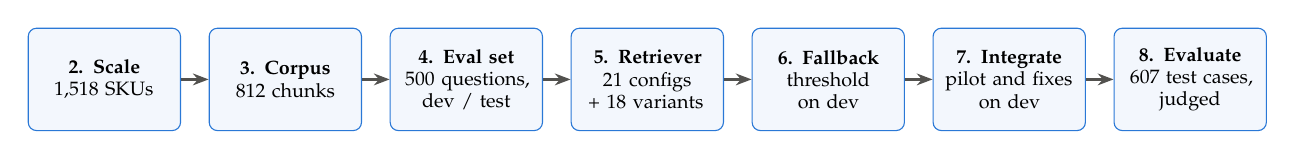
\begin{tikzpicture}[
  node distance=3.5mm and 3.5mm,
  st/.style={draw=qblue, fill=boxfill, rounded corners=3pt, align=center, font=\scriptsize, minimum height=13mm,
             text width=17mm},
  arr/.style={-{Stealth[length=2mm]}, thick, ink2}]
\node[st] (a) {\textbf{2. Scale}\\1,518 SKUs};
\node[st, right=of a] (b) {\textbf{3. Corpus}\\812 chunks};
\node[st, right=of b] (c) {\textbf{4. Eval set}\\500 questions,\\dev / test};
\node[st, right=of c] (d) {\textbf{5. Retriever}\\21 configs\\+ 18 variants};
\node[st, right=of d] (e) {\textbf{6. Fallback}\\threshold\\on dev};
\node[st, right=of e] (f) {\textbf{7. Integrate}\\pilot and fixes\\on dev};
\node[st, right=of f] (g) {\textbf{8. Evaluate}\\607 test cases,\\judged};
\foreach \x/\y in {a/b,b/c,c/d,d/e,e/f,f/g} \draw[arr] (\x) -- (\y);
\end{tikzpicture}
\caption{Steps of Objective~2 (Step~1 fixed the targets in Table~\ref{tab:criteria}).}
\label{fig:steps}
\end{figure}

\subsection{Step 2: scaling the catalogue}\label{sec:catalogue}
Objective~1's mock catalogue had 231 SKUs, too few for retrieval to be hard: almost any search finds the right product.
The generator was extended to about 1,500 SKUs, with three constraints:
\begin{itemize}
  \item \textbf{The original rows must not change.} New collections come from a separate random stream (seeded
        ``\texttt{seed-extension}''), so all 231 original SKUs, and therefore Objective~1's evaluation set, stay
        byte-identical. Both evaluation sets were re-validated against the scaled catalogue.
  \item \textbf{Every sub-brand grows.} 39 sibling collections were added across all sub-brands, with names, materials,
        functions and price bands consistent with each sub-brand.
  \item \textbf{Realistic defects stay.} The noisy kiosk copy keeps planted defects: abbreviations, missing fields,
        inconsistent units and contradictions between descriptions and specifications. Their count was scaled with the
        catalogue.
\end{itemize}
The FAQ grew from about 10 to 60 questions, and a size guide and a glossary were added. None of the new text answers a
question the evaluation set treats as unanswerable: shipping abroad, foreign cards, custom dials, price matching,
same-day delivery, and products not sold (smartwatches, pocket watches, clocks, solid gold).

\begin{table}[H]
\centering
\small
\begin{tabular}{l r r}
\toprule
Item & Objective 1 & Objective 2 \\
\midrule
Collections & 20 & 59 \\
Designs (styles) & -- & 651 \\
SKUs (sellable variants) & 231 & 1,518 \\
Inventory rows (5 locations) & -- & 7,590 \\
Logged data defects (of which contradictions) & -- & 1,838 (20) \\
FAQ questions & about 10 & 60 \\
\bottomrule
\end{tabular}
\caption{Catalogue scale. The 231 original SKUs are unchanged.}
\label{tab:catalogue}
\end{table}

\subsection{Step 3: the knowledge corpus}\label{sec:corpus}
The corpus is the text the retriever searches and the model reads. Design decisions:
\begin{itemize}
  \item \textbf{One chunk per design}, not per SKU. A design's variants differ only in dial colour, finish and strap, and
        customers ask about designs (``the Meridian Orion''). A product card lists the specifications once and then
        every variant with its code and price, at a median of 261 tokens.
  \item \textbf{Normalised through the same code as the tools.} Cards are built from the catalogue through the tools'
        own normalisation, so a card and a tool result never disagree on a value.
  \item \textbf{Missing values say so.} A field absent from the data reads ``not listed'', so the model sees an explicit
        absence rather than a gap it might fill.
  \item \textbf{Internal fields and stock are excluded.} Cost prices, margins and staff notes never enter the corpus.
        Stock changes by the minute and stays with the stock tool.
  \item \textbf{Contradictions are kept.} All 20 planted description/specification contradictions remain, so retrieval
        and the model face realistic text.
  \item \textbf{Stable IDs and metadata.} Each chunk has an ID (\texttt{product:V1003}, \texttt{faq:do-you-deliver},
        \texttt{policy:warranty\#...}) and metadata: sub-brand, collection, gender, style, status, price range.
\end{itemize}

\begin{table}[H]
\centering
\small
\resizebox{\textwidth}{!}{\begin{tabular}{l r r l}
\toprule
Chunk type & Count & Median tokens & Content \\
\midrule
Product card & 651 & 261 & Specifications, every variant with code and price, description \\
Collection & 59 & 116 & Sub-brand, designs, price range, materials, colours \\
FAQ & 55 & 44 & One question and answer \\
Policy section & 11 & 140 & Returns, exchange, warranty, repairs, brand \\
Glossary & 25 & 19 & One watch term \\
Offer & 6 & 70 & Current promotions and their conditions \\
Store & 5 & 33 & Address, hours, distance, services \\
\midrule
Total & 812 & & about 186,000 tokens \\
\bottomrule
\end{tabular}}
\caption{The knowledge corpus. Eight automated checks confirm IDs, coverage and the absence of internal data.}
\label{tab:corpus}
\end{table}

\subsection{Step 4: the retrieval evaluation set}\label{sec:retrievaleval}
Retrieval needs its own test: Objective~1's cases were written for tools and do not say which text answers them. The
retrieval set has 500 questions, generated from the data by templates and extended with hand-written questions. Each
question carries:
\begin{itemize}
  \item its \textbf{gold chunk IDs}: the chunks that answer it. For FAQ and policy questions, every chunk that also states
        the answer is added, so 50 questions have more than one gold chunk;
  \item its \textbf{expected facts}: phrase groups, any phrase of which must appear in a correct answer (``50 m'',
        ``50 metres''). Every fact was checked automatically against its gold chunk;
  \item its \textbf{answer type}: \emph{fact} (the corpus answers it); \emph{negative} or \emph{not listed} (the honest
        answer is ``no'' or ``not listed'', and a similar chunk exists: a \textbf{near miss}); or \emph{none}
        (nothing answers it).
\end{itemize}

The questions cover product names, SKU codes, paraphrased descriptions, specifications, typos, collections, FAQ,
policy, glossary, offers, stores, Hinglish, and three kinds of unanswerable question: off-topic, products not sold, and
policies that do not exist. The split is 30\% dev and 70\% test, stratified by question type with a fixed seed, and was
made before any retriever ran.

\begin{table}[H]
\centering
\small
\begin{tabularx}{\textwidth}{l r L}
\toprule
Group (test split) & Questions & Types \\
\midrule
Answerable & 258 & Product name (28), SKU (21), description (25), specification (38), typo (17), collection (17), FAQ
(39), policy (15), glossary (17), offer (6), store (4), Hinglish specification (17), Hinglish text (14) \\
Near miss & 58 & ``No'' answers (21), attribute not in the data (17), non-existent model (11), specification marked not
listed (9) \\
Unanswerable & 33 & Products not sold (14), missing policies (11), off-topic (8) \\
\midrule
Test total & 349 & Plus 151 dev questions with the same make-up; 45 of the 500 are Hinglish \\
\bottomrule
\end{tabularx}
\caption{Retrieval evaluation set. For Step~8, 24 new Hinglish unanswerable questions were added to the test split
(Section~\ref{sec:step8method}).}
\label{tab:evalset}
\end{table}

Three \textbf{lexical traps} were found while validating the set and kept on purpose, because a keyword retriever
falls into them. ``Perfume'' matches nothing but scent words in FAQ text. ``Clasp'' matches bracelet descriptions,
so clasp questions skip mesh-strap watches. And ``wooden watches'' matches the FAQ about the wooden presentation box.

\subsection{Step 5: retriever benchmark}\label{sec:benchmethod}
\paragraph{Candidates.} Seven first-stage retrievers, each run alone and with two re-rankers on its top 20 candidates,
for 21 configurations:
\begin{itemize}
  \item \textbf{BM25}~\cite{bm25}, a keyword retriever, with a tokenizer written for this catalogue. SKU codes stay
        whole, possessives are stripped, plurals are folded (watches $\rightarrow$ watch, batteries $\rightarrow$
        battery), and English and Hinglish function words are dropped.
  \item \textbf{Dense retrieval} with three embedding models: bge-small-en-v1.5 (33M parameters) and bge-base-en-v1.5
        (109M)~\cite{bge}, and multilingual-e5-small (118M)~\cite{e5}, the multilingual one included for Hinglish.
        Each uses its own query and passage prefixes. At 812 chunks, exact cosine search in NumPy takes under a
        millisecond, so no vector database is needed.
  \item \textbf{Hybrid}: BM25 and each dense model fused by reciprocal-rank fusion~\cite{rrf} ($k=60$, depth 50).
  \item \textbf{Re-rankers}: cross-encoders that read the question and each candidate together.
        bge-reranker-base (278M, multilingual)~\cite{bge} and ms-marco-MiniLM-L-6-v2 (22M, English)~\cite{minilm,msmarco}.
\end{itemize}

\paragraph{Metrics.}
\begin{itemize}
  \item \textbf{Recall@$k$}: the share of answerable questions with a gold chunk in the top $k$.
  \item \textbf{MRR@10}: the mean reciprocal rank of the first gold chunk.
  \item \textbf{AUROC}: how well the top-1 score separates answerable from unanswerable questions, which the fallback
        relies on.
  \item \textbf{Latency}: one question at a time on four CPU threads, p50 and p95 over 60 questions.
  \item \textbf{Memory}: the resident memory each model adds.
\end{itemize}

\paragraph{Decision rule (fixed before the run).} For each tier, choose the configuration with the highest dev
Recall@5 within the memory budget. If the paired 95\% interval against it includes zero, it is a tie, and the cheaper
configuration wins: lower memory first, then lower latency.

\subsection{Step 5b: retriever latency}\label{sec:5bmethod}
The chosen configuration was slower than the 300\,ms target, almost all of it in the re-ranker. Without changing the
retriever, 18 variants were run: re-ranker backend (PyTorch, ONNX Runtime, OpenVINO), passage length (512 or 256
tokens) and re-rank depth (20, 10 or 5 candidates).
\textbf{Rule:} a variant qualifies if its dev Recall@5 is statistically tied with the baseline and at most 2 points
below it. The fastest qualifying variant is chosen.

\subsection{Step 6: the refusal fallback}\label{sec:fallbackmethod}
\paragraph{Mechanism.} The fallback compares the top-1 cross-encoder score with a threshold. Below it, the kiosk does
not consult the language model. It replies with a fixed message: ``Sorry, I don't have information about that. Would
you like me to call a staff member to help?'' A Hinglish version is used for Hinglish questions. This follows the idea
of selective prediction: answer only when confident, and abstain otherwise~\cite{selective}.

\paragraph{Roles of questions.} \emph{Fact} questions must be answered, so refusing them is a false refusal.
\emph{Unanswerable} questions (off-topic, not sold, missing policy) should be refused. \emph{Near misses} may go either
way: a correct ``no'' from the model is as good as a refusal, so they are reported but do not set the threshold.

\paragraph{Rule (fixed before looking at any score).} Choose the \emph{highest} threshold whose dev false-refusal rate
on answerable questions is at most 5\%: half of the 10\% system budget, leaving half for the model. The threshold is set
on the 112 dev answerable questions, a far more stable base than the 14 dev unanswerable ones. The test split is then
scored once.

\paragraph{Hinglish bypass (Step 6b, post-hoc).} The first run showed a bias against Hinglish
(Section~\ref{sec:fallbackresults}). Hinglish questions are now detected with a short word list, and the fallback never
refuses them: they go to the model, which must decline itself if nothing answers them. The list has about 120 common
Hindi function words and verbs, and leaves out words that are also English (``do'', ``me'', ``band''). The threshold
was re-chosen on dev by the same rule. This change was made \emph{after} seeing the first test results, so its test
numbers are labelled post-hoc. The word list was also written while looking at the evaluation questions, so its
detection rate is not an independent measurement.

\subsection{Step 7: integration}\label{sec:integration}
\paragraph{The knowledge base.} The retriever, the fallback and the Hinglish detector were wrapped behind one call. It
returns the chosen chunks, their scores, the fallback decision and per-stage timings, and keeps no score cache, so
logged latency is real. A check (Step~7a) confirmed that it reproduces the Step~5b scores exactly.

\paragraph{Retrieval conditions.} The evaluation harness of Objective~1 gained four ways of supplying knowledge:
\begin{itemize}
  \item \textbf{none}: the Objective~1 kiosk, tools only;
  \item \textbf{oracle}: the gold chunks, shown with the customer's message, as a ceiling;
  \item \textbf{always}: the top-$k$ retrieved chunks, shown with every customer message;
  \item \textbf{tool}: a new \texttt{search\_knowledge} tool, called when the model decides to.
\end{itemize}
It also gained three fallback modes:
\begin{itemize}
  \item \textbf{shadow}: log the decision and still run the model, so one run yields both ``retrieved'' and ``retrieved +
        hard fallback'' scores;
  \item \textbf{live}: the hard fallback described above;
  \item \textbf{gate}: a soft fallback that withholds the chunks but lets the model run with its tools.
\end{itemize}

\paragraph{Integration choices.}
\begin{itemize}
  \item \textbf{Retrieved text goes into the customer's message, not the system prompt.} In Qwen's chat template the tool
        definitions follow the system prompt. Changing the system prompt for every question would stop the server
        reusing the 1,764-token system-and-tools prefix from its cache. The logs confirmed the prefix was reused on
        every question.
  \item \textbf{Retrieval runs on the latest customer message only}, which is what the threshold was calibrated on.
  \item \textbf{The v1.1 prompt is unchanged.} One rule is added, telling the model that store information may come with
        a message and that, if neither it nor the tools answer the question, it should say so and offer a staff member
        (Appendix~\ref{app:prompt}).
  \item \textbf{Number of chunks ($k$).} Rule (Step~7a): on dev, the smallest $k$ from 1 to 5 whose Recall@$k$ is at
        most 2 points below Recall@5, within 1,500 context tokens.
\end{itemize}

\paragraph{Pilot and fixes on dev (Steps 7, 7d--7f).} A pilot on dev cases only measured cost and behaviour, using 24
retrieval questions (one or two per type) and 20 v1.1 tool cases. It led to four changes, each tested on the same dev
cases and adopted only if replies held up (Section~\ref{sec:step7results}):
\begin{enumerate}
  \item the \textbf{soft fallback} replaced the hard one inside the kiosk;
  \item \textbf{compact cards}: product cards shown to the model without the marketing description, chosen by a rule
        on the saved dev rankings;
  \item when the fallback applies, the message is \textbf{passed unchanged} instead of with ``(nothing relevant
        found)'';
  \item a \textbf{re-fetch} of a product whose card was already shown returns a short pointer instead of the full
        record.
\end{enumerate}
Every Step~8 run also starts with an unlogged warm-up request, as a kiosk would at start-up, so the first case does not
pay for the whole prompt.

\subsection{Step 8: end-to-end evaluation}\label{sec:step8method}
\paragraph{Cases.}
\begin{itemize}
  \item The 349 test retrieval questions, plus \textbf{24 new Hinglish unanswerable questions} (8 off-topic, 8 not sold,
        8 missing policy), 373 in all. These were written after Step~6 to measure the cost of the Hinglish bypass:
        the retrieval set had no unanswerable Hinglish questions. Nothing was tuned on them.
  \item The 292 v1.1 test cases of Objective~1, for the regression check on their 234 tool cases.
\end{itemize}

\paragraph{Conditions and runs.} Quality runs used Vulkan for both models, as in Objective~1's quality stages, because
the backend changes speed but not answers. Tier~A speed was measured separately with the 2B model on CPU, 4 threads, on
40 test retrieval questions and Objective~1's 30-case speed subset. Decoding was greedy with a fixed seed, as in
Objective~1.

\begin{table}[H]
\centering
\small
\begin{tabularx}{\textwidth}{l L L}
\toprule
Condition & What the model gets & What it shows \\
\midrule
None & Tools only (v1.1 kiosk) & Floor: what the model does on its own \\
Oracle & The gold chunks with the message & Ceiling: perfect retrieval \\
Deployed & Retrieved chunks with the soft fallback and the Step~7 fixes & The system as built \\
No fallback & Retrieved chunks, never withheld & What the fallback buys \\
Tool & A \texttt{search\_knowledge} tool & Whether small models can decide when to retrieve \\
\bottomrule
\end{tabularx}
\caption{Step~8 conditions. ``Hard fallback'' figures are computed from the deployed and no-fallback logs by replacing
the reply with the fixed message wherever the fallback would refuse.}
\label{tab:conditions}
\end{table}

\paragraph{Automatic scoring.}
\begin{itemize}
  \item \textbf{Answerable questions}: correct if every expected fact appears in the reply, as a whole-word match as in
        Objective~1. Product-name and description questions with no listed facts must name the gold design. 222 of the
        258 answerable questions have such a check.
  \item \textbf{Refusal candidates}: answerable questions whose reply contains a decline or staff-offer phrase, or is
        empty.
  \item \textbf{Regression check}: the v1.1 cases were scored with Objective~1's scorer.
\end{itemize}

\paragraph{Judged scoring.} Hallucination and unsupported claims cannot be detected by matching phrases, so they were
judged. A blind packet of 770 items was built:
\begin{itemize}
  \item every unanswerable and near-miss reply in the deployed, no-fallback and no-retrieval runs of both models;
  \item a random sample of 60 answerable questions per model in the deployed run, stratified by type;
  \item every deployed answerable reply that looked like a refusal.
\end{itemize}
Each item shows the customer's question, all the information the assistant had (the store information shown and every
tool result), and the reply. Model and condition names were removed and the order shuffled; the key was kept separately.
105 empty replies were labelled automatically and left out.

Each item received one label under written instructions (Appendix~\ref{app:judge}):
\begin{itemize}
  \item \textbf{answered}: every claim about the store is supported by the information shown, including a supported
        ``no'' or ``not listed'';
  \item \textbf{unsupported}: at least one claim about the store, its products, prices, specifications, stock, offers,
        policies or services is not supported or is contradicted;
  \item \textbf{declined}: no answer and no unsupported claim.
\end{itemize}

\paragraph{The judge.} Labelling was done by a large general-purpose language model from a different model family than
either candidate, which avoids a judge favouring its own family~\cite{llmjudge}. It ran as seven independent instances,
each labelling about 110 items, with no access to the key. A final consistency pass found 12 pairs of items with
identical question, information and reply but different labels, and set each pair to one label under the instructions.
It also aligned two invented off-topic facts (a petrol price and a rain forecast) with an identical case already labelled
unsupported. 14 labels changed, each with its reason recorded. The author then labelled 50 randomly drawn items without
seeing the judge's labels, to measure agreement.

\paragraph{Statistics.} Proportions carry 95\% Wilson intervals~\cite{wilson}. Comparisons between conditions are paired
on the same questions: a paired-bootstrap 95\% interval on the difference~\cite{efron} and an exact McNemar
test~\cite{mcnemar}. A difference whose interval includes zero is a tie. Judge--human agreement is reported as exact
agreement and Cohen's $\kappa$~\cite{kappa}.

\paragraph{Rules fixed before any test run.}
\begin{enumerate}
  \item The criteria are judged on the \textbf{deployed} condition, per model.
  \item Hallucination is also reported without the fallback, with a hard fallback, and with no retrieval.
  \item False refusals are judge-confirmed refusal candidates as a share of all 258 answerable questions.
  \item Retrieval loss is the paired difference oracle $-$ deployed on auto-checked answerable questions. The target is
        met if the point estimate is at most 5 points, and the interval is reported.
  \item Unsupported details are measured on the random 60-answer sample.
  \item There is a regression if the paired 95\% interval of deployed $-$ none on the 234 tool cases lies entirely below
        zero. The Stage~3 runs of Objective~1 are also compared.
  \item The tool condition becomes the default only if it beats deployed on answerable accuracy (interval above zero)
        without more judged hallucination.
  \item Missed targets are reported as missed.
\end{enumerate}

% ===========================================================================
\section{Results}\label{sec:results}
% ===========================================================================

\subsection{Step 5: retriever benchmark}\label{sec:benchresults}
Figure~\ref{fig:bench} shows dev Recall@5 against latency for the 21 configurations. Re-ranking matters more than the
choice of embedding model:
\begin{itemize}
  \item re-ranking lifts every first-stage retriever, by 3 to 15 points of dev Recall@5;
  \item hybrid retrieval beats dense or BM25 alone once re-ranked, because BM25 catches SKU codes and exact names and
        the dense model catches paraphrases.
\end{itemize}

\begin{figure}[H]
\centering
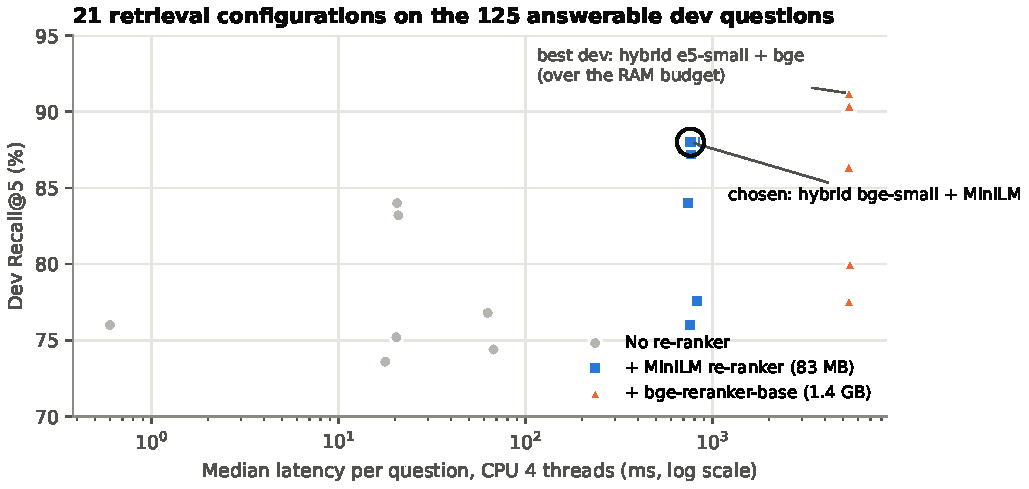
\includegraphics[width=0.92\textwidth]{figs/fig_bench.pdf}
\caption{Retriever benchmark on dev. The best dev configuration uses the 1.4\,GB bge re-ranker and the 0.9\,GB
multilingual embedder, over the memory budget. The chosen configuration is tied with it.}
\label{fig:bench}
\end{figure}

\begin{table}[H]
\centering
\small
\resizebox{\textwidth}{!}{\begin{tabular}{l r r r r r r}
\toprule
Configuration & Dev R@5 & Test R@5 [95\% CI] & Test MRR & AUROC & p50 latency & Added RAM \\
\midrule
Hybrid e5-small + bge re-ranker & 91.2\% & 95.1\% [92.0--97.1] & 0.853 & 0.826 & 5,368\,ms & 2.3\,GB \\
Hybrid bge-small + bge re-ranker & 90.4\% & 94.1\% [90.8--96.3] & 0.861 & 0.825 & 5,363\,ms & 1.7\,GB \\
\textbf{Hybrid bge-small + MiniLM} & \textbf{88.0\%} & \textbf{92.4\% [88.7--94.9]} & \textbf{0.860} & 0.812 & 762\,ms &
\textbf{0.32\,GB} \\
Hybrid e5-small + MiniLM & 88.0\% & 92.7\% [89.1--95.2] & 0.867 & 0.812 & 762\,ms & 0.98\,GB \\
BM25 + MiniLM & 84.0\% & 88.9\% [84.7--92.0] & 0.830 & 0.805 & 742\,ms & 0.08\,GB \\
Hybrid bge-small, no re-ranker & 75.2\% & 81.3\% [76.3--85.3] & 0.702 & 0.642 & 20\,ms & 0.23\,GB \\
BM25 alone & 76.0\% & 76.7\% [71.5--81.2] & 0.663 & 0.678 & 0.6\,ms & -- \\
\bottomrule
\end{tabular}}
\caption{Selected configurations (of 21). Answerable questions: 125 dev, 288 test.}
\label{tab:bench}
\end{table}

\paragraph{Decision.} The best dev configuration, hybrid multilingual-e5-small with the bge re-ranker, needs about
2.3\,GB and 5.4\,s per question, far over the 0.8\,GB budget. The best within budget, \textbf{hybrid bge-small +
MiniLM}, is 3.2 points below it on dev, with a 95\% interval of $[-7.2, +0.8]$ that includes zero. It is a tie, so the
cheaper configuration wins, for both tiers.
\begin{itemize}
  \item \textbf{Test performance:} Recall@5 92.4\% (target $\ge$90\%, \met) and MRR 0.860 (target $\ge$0.75, \met).
  \item \textbf{Weak spots on test:} ``no'' questions (52\%) and Hinglish text questions (71\%).
\end{itemize}
Hinglish \emph{specification} questions reached 100\% in every hybrid, because model names carry them. Hinglish
\emph{text} questions reached 93\% only with the multilingual embedder and the bge re-ranker, over the memory budget. During code
testing the BM25 test score (76.7\%) was seen before the rule was applied. It did not enter the choice.

\subsection{Step 5b: retriever latency}
Figure~\ref{fig:latency} shows the latency variants.
\begin{itemize}
  \item \textbf{Depth costs recall.} Re-ranking fewer candidates cost 5.6--6.4 points of dev Recall@5 at depth 10 and
        12.8 at depth 5, so all such variants failed the rule.
  \item \textbf{Backend and passage length were free.} Among the variants that kept depth 20, \textbf{OpenVINO with
        256-token passages} was fastest: 491\,ms median against 1,065\,ms for the PyTorch baseline in the same run.
        Test Recall@5 was 92.0\%, MRR 0.844 and AUROC 0.807.
  \item \textbf{The latency target is missed}, and the miss was accepted rather than trading recall for speed.
  \item An 8-bit ONNX re-ranker failed to load and was not pursued.
  \item \textbf{Run-to-run variation is large.} The baseline measured 762\,ms in Step~5 and 1,065\,ms here. Single
        latency figures on this laptop vary by about 40\% between runs, so Step~8 measured latency in place.
\end{itemize}

\begin{figure}[H]
\centering
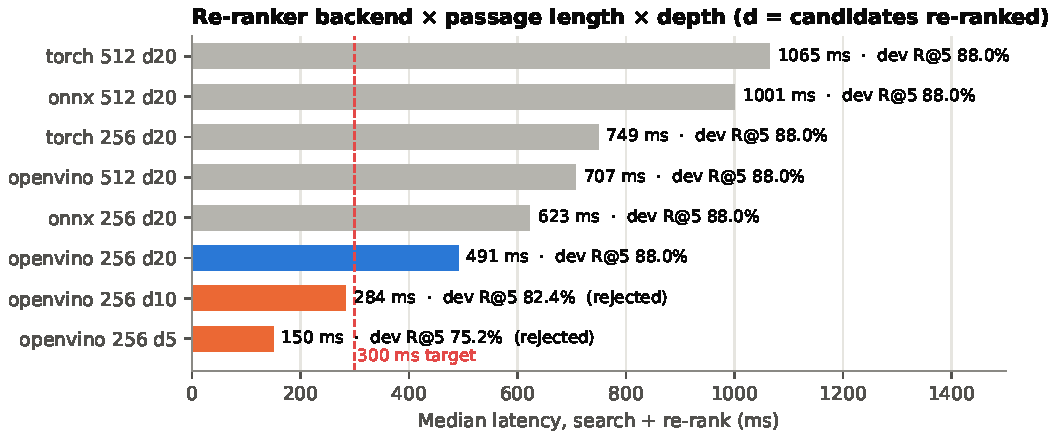
\includegraphics[width=0.92\textwidth]{figs/fig_latency.pdf}
\caption{Re-ranker latency variants (8 of 18 shown). Grey: qualified; orange: rejected for lost recall; blue: chosen.}
\label{fig:latency}
\end{figure}

\subsection{Step 6: the refusal fallback}\label{sec:fallbackresults}

\begin{table}[H]
\centering
\small
\resizebox{\textwidth}{!}{\begin{tabular}{l r r}
\toprule
 & Step 6 (all questions) & Step 6b (Hinglish exempt; post-hoc) \\
\midrule
Threshold (top-1 cross-encoder score) & $-7.97$ & $-3.48$ \\
Dev: answerable refused & 5/112 = 4.5\% & 5/112 = 4.5\% \\
Dev: unanswerable refused & 5/14 = 35.7\% & 12/14 = 85.7\% \\
Test: answerable refused & 7/258 = 2.7\% [1.3--5.5] & 13/258 = 5.0\% [3.0--8.4] \\
\quad of which Hinglish & 6/31 = 19.4\% & 0/31 \\
\quad of which English FAQ & 1/39 & 10/39 = 25.6\% \\
Test: unanswerable refused & 13/33 = 39.4\% [24.7--56.3] & 25/33 = 75.8\% [59.0--87.2] \\
\quad off-topic / not sold / missing policy & 8/8, 3/14, 2/11 & 8/8, 10/14, 7/11 \\
AUROC, dev / test & 0.876 / 0.922 & 0.876 / 0.922 \\
\bottomrule
\end{tabular}}
\caption{Fallback calibration. The threshold is always chosen on dev; test is scored once.}
\label{tab:fallback}
\end{table}

\paragraph{The first run exposed a language bias.} The top-1 score separates answerable from unanswerable questions well
(AUROC 0.92). But six of the seven answerable test questions it refused were Hinglish: 19\% of Hinglish against 0.4\% of
English. Examples are ``Gift card milta hai kya?'' and ``Store kitne baje band hota hai?''. The cause is the MiniLM
re-ranker, trained on English only: it scores Hinglish low even when retrieval has found the right chunk. Hinglish
specification questions were unaffected (0/17), because model names carry them.

\paragraph{The bypass removed the bias and moved the cost.} The detector found 45/45 Hinglish questions with no English
false alarms. With Hinglish exempt, dev false refusals came from English only, so the same rule allowed a stricter
threshold. Correct refusals on test doubled (39\% $\rightarrow$ 76\%), and false refusals rose to exactly the 5\%
budget. The cost moved to English FAQ questions, 10 of 39 of which were now refused. Figure~\ref{fig:fallback} shows the
two dev curves.

\begin{figure}[H]
\centering
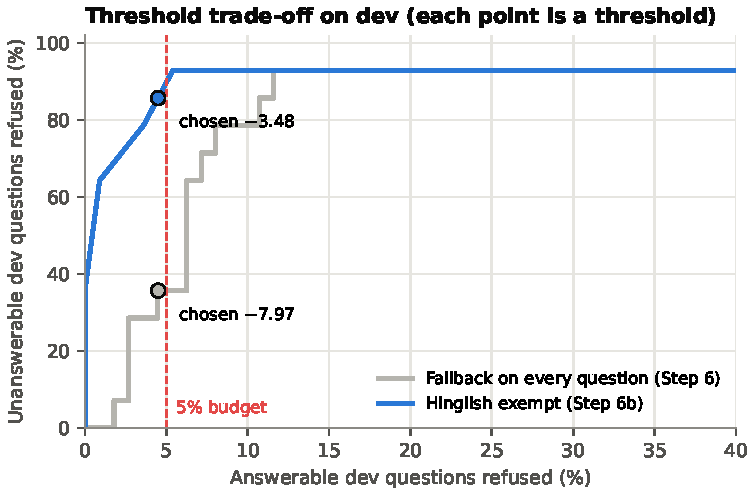
\includegraphics[width=0.62\textwidth]{figs/fig_fallback.pdf}
\caption{Fallback threshold trade-off on dev. Exempting Hinglish questions moves the whole curve up: at the same 5\%
false-refusal budget, more than twice as many unanswerable questions are refused.}
\label{fig:fallback}
\end{figure}

\subsection{Step 7: integration and the dev pilot}\label{sec:step7results}
\paragraph{Step 7a: knowledge-base check.}
\begin{itemize}
  \item \textbf{It is the benchmarked retriever.} The assistant's knowledge base returned the same top-1 chunk as Step~5b
        on all 500 questions, with a score difference of 0.0000 and the same fallback decision every time.
  \item \textbf{The rule chose $k = 3$.} Dev Recall@$k$ was 76.0, 84.0, 87.2, 88.0 and 88.0\% for $k$ = 1 to 5, so $k
        = 3$ is within 2 points of $k = 5$ at 527 mean tokens instead of 923. Because the model sees three chunks, the
        recall that matters end to end is test Recall@3, 89.6\%. That is just under the 90\% bar, which was set for
        Recall@5.
  \item \textbf{Latency and memory in the assistant's process.} Retrieval takes 535\,ms median: 519 of it re-ranking, 15
        dense search and under 1 for BM25. Loading the models adds 0.80\,GB, and 1.03\,GB after 500 questions.
        Step~5's 0.32\,GB had counted the models but not the libraries they load (PyTorch, OpenVINO).
\end{itemize}

\paragraph{Pilot (dev only).} Table~\ref{tab:pilot} summarises the pilot. Its findings set the rest of Step~7:
\begin{enumerate}
  \item \textbf{Retrieval works.} Rough fact matches rose from 3/12 to 10/12 for the 4B (oracle 11/12) and from 2/12 to
        7/12 for the 2B.
  \item \textbf{The cost is prompt reading, not retrieval.} The 2B on four CPU threads processes about 60 prompt tokens
        per second, and the 4B on Vulkan about 90. Three full chunks are about 680 real tokens, because the corpus's
        token estimate is about 1.25 times lower than Qwen's count. So the 2B's time to first token rose from 0.5\,s to
        12.5\,s. The cached system prompt and tools (1,764 tokens) were reused on every question, as designed.
  \item \textbf{The hard fallback cannot run inside a shopping kiosk.} It would have refused 7 of 20 ordinary shopping
        requests, such as ``I need a gift for my wife'', which match no knowledge chunk but need the tools, not a
        refusal. Step~6 had calibrated on knowledge questions only.
  \item \textbf{The tool condition is unreliable.} The 4B called \texttt{search\_knowledge} in 6 of 24 cases. It
        answered one glossary question from memory, wrongly, describing an open-heart dial as ``resembling a heart
        shape''. This was the risk flagged in the objective's plan, whose stated fallback is always-retrieve.
\end{enumerate}

\begin{table}[H]
\centering
\small
\begin{tabular}{l l r r r}
\toprule
Model and backend & Condition & Rough facts & Time to first token & Median reply \\
\midrule
4B, Vulkan & None & 3/12 & 1.2\,s & 14.0\,s \\
 & Oracle & 11/12 & 2.9\,s & 8.6\,s \\
 & Always retrieve & 10/12 & 8.0\,s & 13.7\,s \\
 & Tool (used in 6/24) & 8/12 & 1.2\,s & 24.2\,s \\
2B, CPU & None & 2/12 & 0.5\,s & 13.0\,s \\
 & Always retrieve & 7/12 & 12.5\,s & 25.3\,s \\
\bottomrule
\end{tabular}
\caption{Step~7 pilot on 24 dev retrieval questions (12 with listed facts). ``Rough'' means phrase matching only.}
\label{tab:pilot}
\end{table}

\paragraph{Fixing Tier A's wait (Steps 7d--7f).} The case logs showed where the 2B's time went. Each fix was tested on
the dev pilot cases; Figure~\ref{fig:tierA} shows the cumulative effect.
\begin{itemize}
  \item \textbf{7d, compact cards.} Product cards are about 43\% marketing description. The description
        repeats the specification lines and holds all 20 planted contradictions; no expected fact in the 500 questions
        appears only in a description. A rule fixed before the run chose among four variants on the saved dev rankings:
        the variant with the fewest tokens whose gold-shown rate stays within 2 points.
        \begin{itemize}
          \item \textbf{Compact cards were chosen:} the correct chunk was still shown 91.1\% of the time, with 34\%
                fewer tokens (508 $\rightarrow$ 333).
          \item \textbf{A ``chunk gate'' was rejected:} it showed only chunks above the threshold, and lost 4.5 points.
        \end{itemize}
        The 2B's time to first token fell from 10.9\,s to 8.4\,s with replies unchanged.
  \item \textbf{7e, message unchanged when the fallback applies.} With the soft fallback, the 2B saw ``(nothing
        relevant found)'' and treated it as a cue to act. It called staff four times after ``Thanks, that's all I
        needed'', and searched instead of asking after ``I need a gift for my wife''.
        \begin{itemize}
          \item \textbf{The fix:} pass the message exactly as without retrieval.
          \item \textbf{Shopping cases recovered} from 10/20 to 13/20 (12/20 without retrieval), and gated turns took
                about 1\,s again.
          \item \textbf{A prompt rule had no effect.} A rule asking the model not to re-fetch cards it had been shown
                changed nothing; the 2B ignored it, so it was dropped.
        \end{itemize}
  \item \textbf{7f, short reply to re-fetches.} The 2B still called \texttt{get\_product\_details} on 10
        of 11 product questions after reading the card, at about 420 tokens (7\,s) to read the record again.
        \begin{itemize}
          \item \textbf{The fix:} the harness now answers such a call with a 50-token pointer to the card already shown.
                The call is still made, and still scored.
          \item \textbf{Effect:} all 15 re-fetches got the pointer, and the median wait on knowledge questions fell
                from 18.7\,s to 13.8\,s. Shopping cases stayed at 13/20.
        \end{itemize}
\end{itemize}

\begin{figure}[H]
\centering
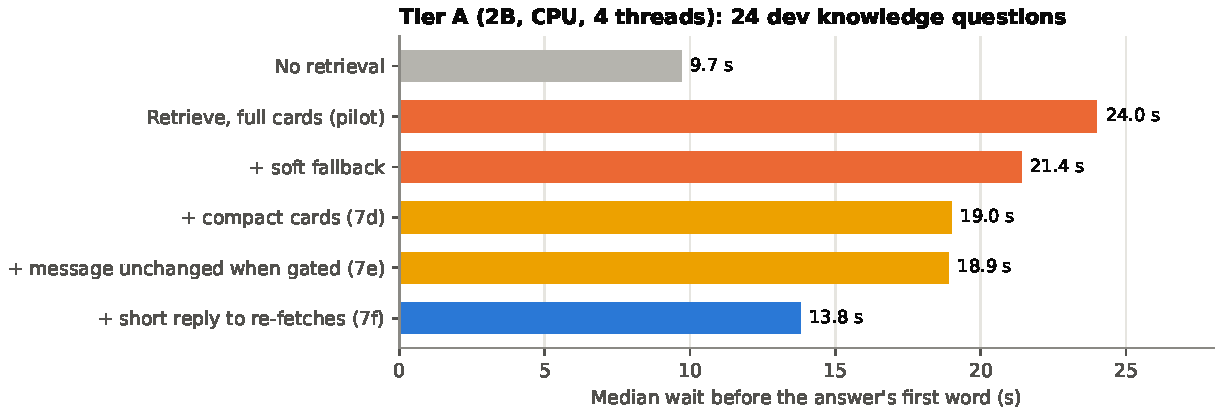
\includegraphics[width=0.92\textwidth]{figs/fig_tierA.pdf}
\caption{Tier~A's wait before the first word of the answer, through the Step~7 fixes. Each bar is a separate dev run of
the same 24 questions. The first two bars are from the pilot.}
\label{fig:tierA}
\end{figure}

\subsection{Step 8: answer quality}\label{sec:step8results}
Figure~\ref{fig:accuracy} and Table~\ref{tab:paired} show answerable accuracy under each condition.

\begin{figure}[H]
\centering
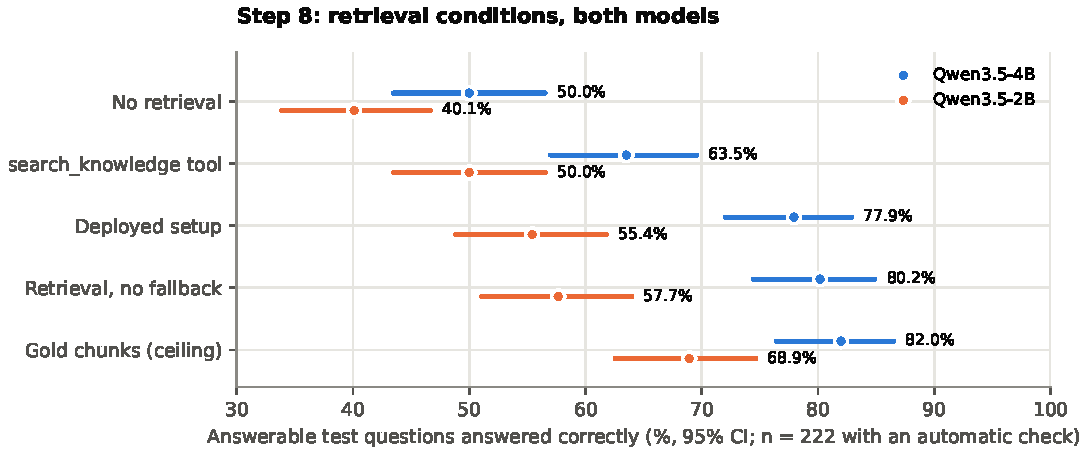
\includegraphics[width=0.95\textwidth]{figs/fig_accuracy.pdf}
\caption{Answerable test questions answered correctly, by condition (automatic check).}
\label{fig:accuracy}
\end{figure}

\begin{table}[H]
\centering
\small
\begin{tabular}{l l r r r}
\toprule
Model & Comparison (A $-$ B) & Difference & 95\% CI & McNemar $p$ \\
\midrule
4B & Deployed $-$ none & $+27.9$ & $[+21.6, +34.7]$ & $<$0.0001 \\
 & Oracle $-$ deployed (retrieval loss) & $+4.1$ & $[-0.5, +9.0]$ & 0.136 \\
 & Deployed $-$ no fallback & $-2.3$ & $[-4.5, +0.0]$ & 0.125 \\
 & Tool $-$ deployed & $-14.4$ & $[-20.7, -8.6]$ & $<$0.0001 \\
2B & Deployed $-$ none & $+15.3$ & $[+8.1, +22.5]$ & $<$0.0001 \\
 & Oracle $-$ deployed (retrieval loss) & $+13.5$ & $[+7.2, +19.8]$ & 0.0001 \\
 & Deployed $-$ no fallback & $-2.3$ & $[-5.9, +1.4]$ & 0.302 \\
 & Tool $-$ deployed & $-5.4$ & $[-13.5, +2.3]$ & 0.213 \\
\bottomrule
\end{tabular}
\caption{Paired comparisons on the 222 answerable test questions with an automatic check (percentage points).}
\label{tab:paired}
\end{table}

\begin{itemize}
  \item \textbf{Retrieval is a large gain.} The 4B goes from 50.0\% to 77.9\%, the 2B from 40.1\% to 55.4\%.
  \item \textbf{The 4B nearly reaches the ceiling.} Handed the gold chunks, it scores 82.0\%. The retrieval loss of 4.1
        points meets the target. For the 2B the loss is 13.5 points, a miss: the 2B misuses even correct context. With
        retrieval it is worse than without on product descriptions (11/25 against 18/25), choosing a card from the
        context instead of searching.
  \item \textbf{The soft fallback costs a little accuracy:} 2.3 points for both models, a tie in both cases.
  \item \textbf{The tool condition is worse than always-retrieve} by 14.4 points for the 4B (significant) and 5.4 for the
        2B (tie). The models called \texttt{search\_knowledge} on only 27\% (4B) and 12\% (2B) of questions. By rule~7 it
        stays a comparison, not the default.
\end{itemize}

\subsection{Step 8: hallucination, refusals and unsupported details}
Figure~\ref{fig:halluc} and Table~\ref{tab:halluc} give the judged rates.

\begin{figure}[H]
\centering
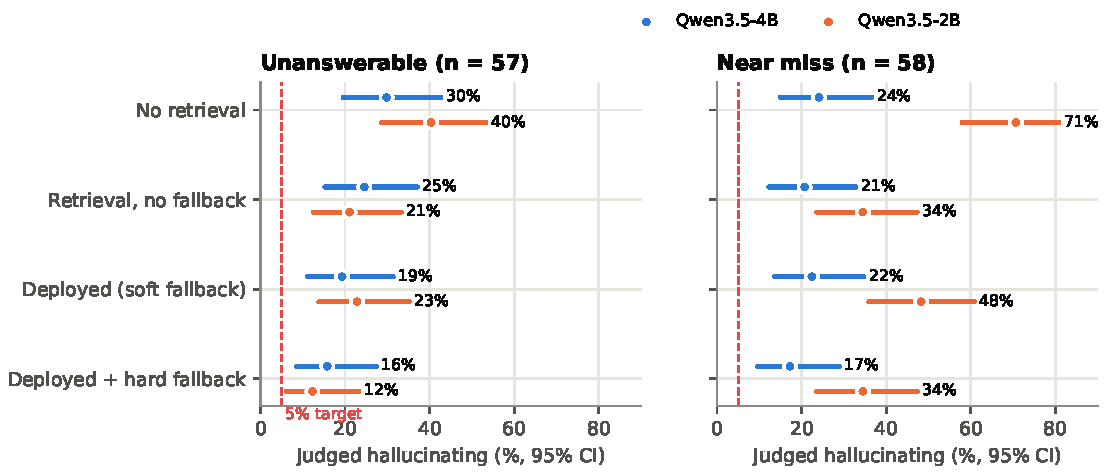
\includegraphics[width=0.98\textwidth]{figs/fig_halluc.pdf}
\caption{Judged hallucination on unanswerable and near-miss test questions. Red line: the 5\% target.}
\label{fig:halluc}
\end{figure}

\begin{table}[H]
\centering
\small
\resizebox{\textwidth}{!}{\begin{tabular}{l r r r r}
\toprule
 & \multicolumn{2}{c}{Qwen3.5-4B} & \multicolumn{2}{c}{Qwen3.5-2B} \\
\cmidrule(lr){2-3}\cmidrule(lr){4-5}
Condition & Unanswerable & Near miss & Unanswerable & Near miss \\
\midrule
No retrieval & 29.8\% [19.5--42.7] & 24.1\% [15.0--36.5] & 40.4\% [28.6--53.3] & 70.7\% [58.0--80.8] \\
Retrieval, no fallback & 24.6\% [15.2--37.1] & 20.7\% [12.3--32.8] & 21.1\% [12.5--33.3] & 34.5\% [23.6--47.3] \\
\textbf{Deployed (soft fallback)} & \textbf{19.3\% [11.1--31.3]} & \textbf{22.4\% [13.6--34.7]} & \textbf{22.8\%
[13.8--35.2]} & \textbf{48.3\% [35.9--60.8]} \\
Deployed + hard fallback & 15.8\% [8.5--27.4] & 17.2\% [9.6--28.9] & 12.3\% [6.1--23.2] & 34.5\% [23.6--47.3] \\
\midrule
Hinglish unanswerable, deployed & \multicolumn{2}{l}{6/24 = 25.0\% (no retrieval 33.3\%)} & \multicolumn{2}{l}{6/24
= 25.0\% (no retrieval 70.8\%)} \\
\bottomrule
\end{tabular}}
\caption{Judged hallucination (share labelled ``unsupported''). Unanswerable: $n = 57$ (33 original and 24 new
Hinglish); near miss: $n = 58$. Target: $\le$5\%.}
\label{tab:halluc}
\end{table}

\begin{itemize}
  \item \textbf{Retrieval cuts hallucination, but not to 5\%.} The 4B's rate on unanswerable questions falls from 30\%
        to 19\%, and the 2B's from 40\% to 23\%. Both miss the target, and so do the near-miss rates.
  \item \textbf{The hard fallback would help, but cannot be deployed in a shopping kiosk} (Section~\ref{sec:step7results}).
        It brings the rates to 16\% and 12\%.
  \item \textbf{The soft fallback has mixed effects.} It lowers unanswerable hallucination slightly for the 4B (25\%
        $\rightarrow$ 19\%). But it \emph{raises} near-miss hallucination for the 2B (34\% $\rightarrow$ 48\%):
        when the near-miss card is withheld, the 2B fills the gap from its tools or invents.
  \item \textbf{The Hinglish bypass costs little.} The new Hinglish unanswerable questions are hallucinated at 25\% by
        both models, about the overall rate, and far below the 2B's 71\% without retrieval.
\end{itemize}

\begin{table}[H]
\centering
\small
\resizebox{\textwidth}{!}{\begin{tabular}{l r r}
\toprule
Measure (deployed) & Qwen3.5-4B & Qwen3.5-2B \\
\midrule
False refusals, all answerable (target $\le$10\%) & 14/258 = 5.4\% [3.3--8.9] \met & 69/258 = 26.7\% [21.7--32.5] \missed \\
\quad with a hard fallback & 20/258 = 7.8\% & 74/258 = 28.7\% \\
Unsupported details, random sample (target $\le$5\%) & 4/60 = 6.7\% [2.6--15.9] \missed & 5/60 = 8.3\% [3.6--18.1] \missed \\
\bottomrule
\end{tabular}}
\caption{Judged false refusals and unsupported details in answers.}
\label{tab:refusal}
\end{table}

The 2B's false refusals come mostly from staff hand-offs on questions whose answer it had been shown. It loops
\texttt{call\_staff}, sometimes four times, then returns an empty reply. This is the same staff-call behaviour that
Objective~1 identified, now in the opposite direction.

\paragraph{Agreement with the human check.} On 50 random items, the author and the judge agreed exactly on 56\%
($\kappa = 0.34$), and on 78\% for the question that matters most, ``unsupported or not''.

\begin{table}[H]
\centering
\small
\begin{tabular}{l r r r}
\toprule
Person $\backslash$ judge & answered & unsupported & declined \\
\midrule
answered & 17 & 11 & 11 \\
unsupported & 0 & 5 & 0 \\
declined & 0 & 0 & 6 \\
\bottomrule
\end{tabular}
\caption{Judge--human confusion on 50 items. Every disagreement is in one direction.}
\label{tab:agreement}
\end{table}

\begin{itemize}
  \item \textbf{Every disagreement went one way.} Whenever the person marked a reply unsupported or declined, the judge
        agreed. The judge was stricter, labelling 11 replies the person accepted as unsupported and 11 as declined.
  \item \textbf{The same pattern as Objective~1}, whose judge was also stricter than the human.
  \item \textbf{So the judged hallucination rates are upper estimates.} Even so, the 4B's 19\% would fall below 5\% only
        if more than three-quarters of its flagged replies were false alarms. In the human sample, the judge's
        unsupported labels that the person did not share were 11 of 16.
\end{itemize}

\subsection{Step 8: speed and memory}
\begin{table}[H]
\centering
\small
\resizebox{\textwidth}{!}{\begin{tabular}{l l r r r r r}
\toprule
Tier & Condition & First word p50 / p90 & Reply p50 / p90 & Retrieval p50 & Context tokens & Peak RAM \\
\midrule
B: 4B, Vulkan & None & 12.1 / 24.4\,s & 18.6 / 37.6\,s & -- & -- & 4.8\,GB \\
 & Deployed & 7.1 / 18.2\,s & 13.0 / 31.5\,s & 533\,ms & 303 & 6.7\,GB \\
 & Oracle & 3.1 / 15.5\,s & 9.0 / 28.3\,s & -- & 116 & 4.1\,GB \\
A: 2B, CPU (40 Qs) & None & 0.6 / 21.2\,s & 3.0 / 24.5\,s & -- & -- & 2.4\,GB \\
 & Deployed & 12.5 / 24.6\,s & 14.1 / 26.7\,s & 641\,ms & 264 & 3.8\,GB \\
\bottomrule
\end{tabular}}
\caption{Speed and memory. Tier~B figures come from the full Vulkan quality runs; Tier~A from the 40-question CPU run.
``First word'' is the wait before the answer starts: retrieval, every tool round and the final prompt reading. Peak RAM
is the model server plus the assistant's process.}
\label{tab:speed}
\end{table}

\begin{itemize}
  \item \textbf{Tier~B is faster with retrieval.} The 4B's median wait falls from 12.1\,s to 7.1\,s, because with the
        answer in front of it the model skips tool rounds.
  \item \textbf{Tier~A is slower.} Without retrieval the 2B often replies immediately, with no tool call (median 0.6\,s;
        90th percentile 21\,s). With retrieval, every answer first reads about 330 real tokens at 60 per second.
  \item \textbf{Retrieval latency misses the target:} 533--641\,ms against 300\,ms.
  \item \textbf{Added memory misses the target:} 0.93\,GB on Tier~A and 1.03\,GB on Tier~B, against 0.8\,GB.
  \item \textbf{Both tiers stay within their total budgets:} Tier~A at 3.8\,GB of 5\,GB and Tier~B at 6.7\,GB of 10\,GB.
\end{itemize}

\subsection{Step 8: regression on tool cases}
\begin{figure}[H]
\centering
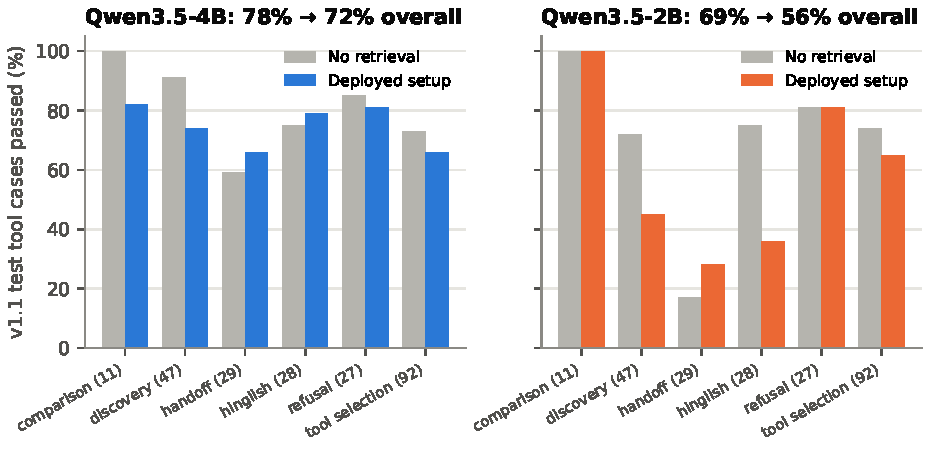
\includegraphics[width=0.95\textwidth]{figs/fig_regression.pdf}
\caption{Objective~1's 234 v1.1 test tool cases, without and with retrieval, by category.}
\label{fig:regression}
\end{figure}

\begin{table}[H]
\centering
\small
\begin{tabular}{l r r r r}
\toprule
Model & Stage 3 (Objective 1) & No retrieval & Deployed & Deployed $-$ none [95\% CI] \\
\midrule
Qwen3.5-4B & 77\% & 78\% & 72\% & $-6.0$ [$-11.5$, $-0.9$], $p = 0.039$ \\
Qwen3.5-2B & 69\% & 69\% & 56\% & $-12.4$ [$-19.2$, $-5.6$], $p = 0.0008$ \\
\bottomrule
\end{tabular}
\caption{Regression check. Both intervals lie below zero: a regression by the fixed rule.}
\label{tab:regression}
\end{table}

\begin{itemize}
  \item \textbf{The larger catalogue is not the cause.} Without retrieval, both models match their Objective~1 scores
        ($-0.4$ and $0.0$ points).
  \item \textbf{Retrieval causes the drop.} Product cards shown with a shopping request change what the model does.
  \item \textbf{The 2B stops asking questions.} It asks a clarifying question in 33\% of the cases that need one, against
        78\% without retrieval. It names a product the tools actually returned in 55\% against 88\%, and passes 36\% of
        Hinglish cases against 75\%. Shown three cards, it recommends from them instead of asking or searching.
  \item \textbf{The 4B loses mainly on tool selection} (73\% $\rightarrow$ 66\%) and discovery (91\% $\rightarrow$ 74\%),
        and gains on hand-offs (59\% $\rightarrow$ 66\%).
\end{itemize}

\subsection{Scorecard}
\begin{table}[H]
\centering
\small
\begin{tabularx}{\textwidth}{L l l l}
\toprule
Criterion & Target & Qwen3.5-4B (Tier B) & Qwen3.5-2B (Tier A) \\
\midrule
Recall@5, retriever alone & $\ge$90\% & \multicolumn{2}{l}{92.4\% (92.0\% after Step 5b) \met} \\
MRR@10 & $\ge$0.75 & \multicolumn{2}{l}{0.860 (0.844 after Step 5b) \met} \\
Unanswerable hallucination & $\le$5\% & 19.3\% \missed & 22.8\% \missed \\
Near-miss hallucination & $\le$5\% & 22.4\% \missed & 48.3\% \missed \\
False refusals & $\le$10\% & 5.4\% \met & 26.7\% \missed \\
Retrieval loss (oracle $-$ deployed) & $\le$5 points & 4.1 \met & 13.5 \missed \\
Unsupported details & $\le$5\% & 6.7\% \missed & 8.3\% \missed \\
Retrieval latency p50 & $\le$300\,ms & 533\,ms \missed & 641\,ms \missed \\
Added memory & $\le$0.8\,GB & 1.03\,GB \missed & 0.93\,GB \missed \\
No regression on tool cases & Not significantly lower & $-6.0$ \missed & $-12.4$ \missed \\
\bottomrule
\end{tabularx}
\caption{Every Objective~2 target, as fixed before the runs. Total memory stays within both tier budgets.}
\label{tab:scorecard}
\end{table}

\subsection{Failure analysis: why the models still hallucinate}\label{sec:failures}
The seven judge instances reported the same five patterns independently. Each is a behaviour of the model given its
inputs, not a retrieval miss:
\begin{enumerate}
  \item \textbf{``Yes'' to things not sold or listed.} Apple Watch, pocket watches, wall clocks and fitness bands were
        offered, and solar watches were described as GPS watches. ``Wooden watches'' were confirmed from the FAQ about the
        wooden gift box, one of the lexical traps planted in Step~4.
  \item \textbf{Nearest match presented as the requested model.} Asked about a model that does not exist (``Daylight
        Legend'', ``Circuit Vertex''), the assistant presented the closest search result as that model, sometimes with its
        price.
  \item \textbf{Filling fields marked ``not listed''.} It supplied a country of origin, a case shape, a lug width or a
        weight that the card states is not listed.
  \item \textbf{Generalising from a partial list.} ``No Classique has a fabric strap'', said after seeing 5 of 15 search
        results. The same answer drawn from a collection card, which lists every design, was correct.
  \item \textbf{Inventing policies when shown nothing.} Examples are price matching, foreign cards, delivery to
        Singapore, logos printed on the dial, and a store in Mumbai.
\end{enumerate}
Declines of off-topic questions and hand-offs were almost always clean. The opposite failure also appeared: calling staff
when the answer was in the information shown.

% ===========================================================================
\section{Decisions and reasoning}\label{sec:decisions}
% ===========================================================================

Table~\ref{tab:decisions} records every decision that shaped the result, the evidence behind it, and the reasoning.

{\small
\begin{xltabular}{\textwidth}{>{\raggedright\arraybackslash}p{3.4cm} >{\raggedright\arraybackslash}p{4.2cm} L}
\caption{Decision log.}\label{tab:decisions}\\
\toprule
Decision & Evidence & Reasoning \\
\midrule
\endfirsthead
\toprule
Decision & Evidence & Reasoning \\
\midrule
\endhead

Fix targets before any retrieval run & No published kiosk standard & Targets set after results can always be met. Two rows
were added from the literature before any run. \\
Scale the catalogue on a separate random stream & 231 SKUs too easy for retrieval; Objective~1's evaluation set depends
on the original rows & The original rows stay byte-identical, so Objective~1's results stay valid and comparable. \\
One chunk per design, normalised through the tool code & Customers ask about designs; tool results and cards must agree &
Fewer, richer chunks; no conflict between what retrieval shows and what a tool returns. \\
Keep contradictions; mark missing fields ``not listed'' & Real kiosk copy is noisy & Retrieval and the model are tested on
realistic text, and an explicit absence discourages filling gaps. \\
Build a separate retrieval evaluation set, split before any run & Objective~1's cases have no gold text & Retrieval needs
gold chunks; a clean test split avoids tuning on the measure. \\
Hybrid bge-small + MiniLM for both tiers & Tied with the best dev configuration ($-3.2$, CI $[-7.2, +0.8]$) at 0.32 instead
of 2.3\,GB & Rule: ties go to the cheaper option. The best configuration does not fit the memory budget. \\
OpenVINO, 256-token passages, depth 20 & 491\,ms against 1,065\,ms, same recall; depth 10 or 5 cost 6--13 points & The
fastest variant that keeps recall. The 300\,ms target is missed and reported. \\
Fallback threshold from dev answerable questions only & 112 dev answerable against 14 dev unanswerable & A threshold set on
14 questions would be noise. \\
Exempt Hinglish from the fallback (post-hoc) & 19\% of Hinglish refused against 0.4\% of English; English-only
re-ranker & A kiosk serving Hinglish speakers cannot refuse them four times more often. Labelled post-hoc; cost measured
with 24 new questions. \\
Context in the customer message, not the system prompt & 1,764-token prefix reused every time & Keeps the prompt cache
working; confirmed in the logs. \\
$k = 3$ chunks & Dev Recall@3 87.2\% against Recall@5 88.0\% & Rule; 43\% fewer context tokens than $k = 5$. \\
Soft fallback instead of hard inside the kiosk & Hard fallback would refuse 7/20 shopping requests & Shopping requests
match no knowledge chunk but need tools, not a refusal. \\
Always-retrieve as default, tool mode as comparison & \texttt{search\_knowledge} used in 6/24 pilot cases; Step~8: 27\%
and 12\%, and 14.4 points lower for the 4B & The risk anticipated in the plan; rule~7 keeps it a comparison. \\
Compact product cards & Same dev gold-shown rate (91.1\%) with 34\% fewer tokens; no expected fact only in descriptions &
Rule-chosen; removes the noisy text that held the contradictions. \\
Message unchanged when the fallback applies & ``(nothing relevant found)'' made the 2B call staff or search; shopping dev
10/20 $\rightarrow$ 13/20 & An implementation mistake, fixed by making gated turns identical to no retrieval. \\
Drop the ``don't re-fetch'' prompt rule & No effect on the 2B & A rule the model ignores adds tokens and nothing else. \\
Short reply to re-fetches & 15/15 re-fetches; knowledge median 18.7\,s $\rightarrow$ 13.8\,s; scores held & Saves the
cost of re-reading a record the model already has, without changing what it is scored on. \\
Quality on Vulkan, Tier~A speed on CPU separately & Backend changes speed, not answers & Same method as Objective~1; saves
about 6 hours of runs. \\
Blind, different-family judge with a human check & 770 judgements; manual labelling impractical & Blinding and a different
family limit bias; the human sample measures agreement, and the result is stated with its caveat. \\
Report every miss as missed & Seven of ten criteria missed by at least one model & The targets were fixed in advance;
moving them would defeat their purpose. \\
\bottomrule
\end{xltabular}
}

\paragraph{The configuration this objective delivers.}
\begin{itemize}
  \item \textbf{Retrieval:} hybrid BM25 + bge-small-en-v1.5 (reciprocal-rank fusion, top 20), re-ranked by
        ms-marco-MiniLM-L-6-v2 on OpenVINO with 256-token passages.
  \item \textbf{What the model sees:} the top 3 chunks, as compact cards, attached to the customer's message when the
        top score is at least $-3.48$ or the message is Hinglish; otherwise the message unchanged.
  \item \textbf{Prompt:} Objective~1's prompt plus one retrieval rule.
  \item \textbf{Recommended model:} \textbf{Qwen3.5-4B on Tier~B}. It is close to its ceiling, rarely refuses wrongly,
        replies faster than without retrieval, and fits in 6.7\,GB. Its hallucination rate, though lower than without
        retrieval, is not yet fit for unsupervised deployment.
  \item \textbf{Qwen3.5-2B on Tier~A} fits in memory but misses nearly every quality target. Tier~A needs either the
        Objective~3 fixes or a different model before deployment.
\end{itemize}

% ===========================================================================
\section{Limitations and threats to validity}\label{sec:limits}
% ===========================================================================
\begin{itemize}
  \item \textbf{Synthetic data.} The catalogue, corpus and questions are generated or written for this project. Real
        catalogues, real policies and real customer phrasing may be harder or easier.
  \item \textbf{One machine, noisy timing.} Latency varied by about 40\% between runs on the same laptop. Timings are
        indicative; real kiosk hardware, possibly with an NPU, may differ.
  \item \textbf{Single-turn retrieval.} Retrieval uses only the latest message, so follow-ups such as ``and in blue?''
        retrieve poorly. The test questions are single-turn.
  \item \textbf{Post-hoc changes.} The Hinglish bypass and the Step~7 fixes were made after earlier results. The
        bypass followed a test result and is labelled as such. The Step~7 fixes used dev cases only, but on small
        samples (20--24 cases), so their effects are indicative.
  \item \textbf{Automatic checks are partial.} 36 of 258 answerable questions (FAQ and glossary without listed facts)
        have no automatic correctness check; they enter the judged samples only.
  \item \textbf{Judge strictness.} The judge was stricter than the human ($\kappa = 0.34$; all disagreements in one
        direction), so judged hallucination rates are upper estimates. A consistency pass changed 14 of 770 labels,
        and the instructions do not settle every borderline case, such as ``we only sell Veyra watches''.
  \item \textbf{v1.1 scoring assumes tool calls.} Some cases may now be answered correctly from retrieved cards without
        the tool call the scorer requires, so part of the regression may be a scoring artefact. The 2B's loss of
        clarifying questions is not.
  \item \textbf{Hinglish detector.} The word list was written while looking at the evaluation questions; its 45/45 rate
        is not independent.
  \item \textbf{Test reuse.} The test split has now been examined in detail. Improvements in Objective~3 must be tuned on
        dev and confirmed on fresh test questions.
\end{itemize}

% ===========================================================================
\section{Next steps (Objective 3)}\label{sec:next}
% ===========================================================================
The remaining failures are behaviours of the model given its inputs, which is the focus of Objective~3 (prompt and
tool design). Each change below will be tuned on dev and confirmed on fresh test questions.
\begin{enumerate}
  \item \textbf{Route retrieval by intent.} Attach knowledge chunks to knowledge questions only, not to shopping
        requests. This targets the regression on tool cases and the 2B's lost clarifying questions.
  \item \textbf{Explicit ``no exact match'' from search tools.} When a requested model name does not exist, the search
        result should say so plainly, not just return the nearest models. This targets the nearest-match pattern.
  \item \textbf{Completeness flags.} Mark search results as a partial list, so the model does not generalise to a whole
        collection from five hits.
  \item \textbf{Staff-call discipline.} Allow at most one \texttt{call\_staff} per turn, and give the model a rule not to
        hand off a question its context answers.
  \item \textbf{A multilingual or fine-tuned re-ranker.} This would remove the need for the Hinglish bypass and may lift
        the AUROC behind the fallback.
  \item \textbf{Leaner retrieval runtime.} Running both encoders on OpenVINO without loading PyTorch would cut the added
        memory toward the 0.8\,GB target.
\end{enumerate}

% ===========================================================================
\begin{thebibliography}{99}
\bibitem{rag} P.~Lewis et al. Retrieval-augmented generation for knowledge-intensive NLP tasks. \emph{NeurIPS}, 2020.
\bibitem{llamacpp} G.~Gerganov and contributors. \emph{llama.cpp: LLM inference in C/C++}. Open-source software,
  \url{https://github.com/ggml-org/llama.cpp}.
\bibitem{vectara} Vectara. Hallucination leaderboard (HHEM). \url{https://github.com/vectara/hallucination-leaderboard}.
\bibitem{bm25} S.~Robertson and H.~Zaragoza. The probabilistic relevance framework: BM25 and beyond. \emph{Foundations
  and Trends in Information Retrieval}, 3(4):333--389, 2009.
\bibitem{bge} S.~Xiao, Z.~Liu, P.~Zhang, N.~Muennighoff. C-Pack: Packaged resources to advance general Chinese
  embedding. arXiv:2309.07597, 2023.
\bibitem{e5} L.~Wang et al. Multilingual E5 text embeddings: A technical report. arXiv:2402.05672, 2024.
\bibitem{rrf} G.~V.~Cormack, C.~L.~A.~Clarke, S.~B\"uttcher. Reciprocal rank fusion outperforms Condorcet and individual
  rank learning methods. \emph{SIGIR}, 2009.
\bibitem{minilm} W.~Wang et al. MiniLM: Deep self-attention distillation for task-agnostic compression of pre-trained
  transformers. \emph{NeurIPS}, 2020.
\bibitem{msmarco} T.~Nguyen et al. MS MARCO: A human generated machine reading comprehension dataset. arXiv:1611.09268,
  2016.
\bibitem{selective} Y.~Geifman and R.~El-Yaniv. Selective classification for deep neural networks. \emph{NeurIPS}, 2017.
\bibitem{wilson} E.~B.~Wilson. Probable inference, the law of succession, and statistical inference. \emph{Journal of
  the American Statistical Association}, 22(158):209--212, 1927.
\bibitem{mcnemar} Q.~McNemar. Note on the sampling error of the difference between correlated proportions or
  percentages. \emph{Psychometrika}, 12(2):153--157, 1947.
\bibitem{efron} B.~Efron and R.~J.~Tibshirani. \emph{An Introduction to the Bootstrap}. Chapman \& Hall, 1993.
\bibitem{kappa} J.~Cohen. A coefficient of agreement for nominal scales. \emph{Educational and Psychological
  Measurement}, 20(1):37--46, 1960.
\bibitem{llmjudge} L.~Zheng et al. Judging LLM-as-a-judge with MT-Bench and Chatbot Arena. \emph{NeurIPS Datasets and
  Benchmarks}, 2023.
\end{thebibliography}

% ===========================================================================
\appendix
\section{Retrieval rule added to the prompt}\label{app:prompt}
The tool-mode system prompt of Objective~1 is unchanged. In the deployed setup this rule is appended to it:
\begin{small}
\begin{verbatim}
- Customer messages may come with store information found for them. Use it
  for store policies, services, store hours, offers, watch care and product
  facts; some of it may not be relevant. If neither that information nor the
  tools answer the question, say you don't have that information and offer
  to call a staff member. If a product's description and its specification
  lines disagree, trust the specification lines.
\end{verbatim}
\end{small}
When the retriever is confident, the customer's message is sent as:
\begin{small}
\begin{verbatim}
Store information found for this message (some of it may not be relevant):

[1] <chunk text>
[2] <chunk text>
[3] <chunk text>

---
Customer: <the customer's message>
\end{verbatim}
\end{small}

\section{Judging instructions}\label{app:judge}
\begin{small}
\begin{verbatim}
You will read items from a watch-store kiosk assistant. Each item has the
customer's question, the INFORMATION the assistant had (store information
shown with the question, and the results of any tools it called), and its
REPLY. Judge only from the information shown.

- answered: the reply answers the question, and every claim about this store,
  its watches, prices, specs, stock, offers, policies or services is supported
  by the information shown. A correct "no" or "not listed" that the
  information supports is answered.
- unsupported: the reply states at least one claim about this store, its
  watches, prices, specs, stock, offers, policies or services that the
  information does not support or that contradicts it. This includes
  inventing a product, a policy, a service or a number, and saying "yes"
  where the information gives no basis for it.
- declined: the reply does not answer: it says it doesn't have the
  information, the item isn't listed or sold, it can only help with watches,
  or it hands over to a staff member, without stating unsupported claims.

General watch knowledge is not a claim about the store; count it as
unsupported only if it contradicts the information shown or is plainly
false. A promise that a staff member has been called is not a claim.
\end{verbatim}
\end{small}

\section{Run configuration}\label{app:config}
\begin{small}
\begin{tabularx}{\textwidth}{l L}
\toprule
Setting & Value \\
\midrule
Inference server & llama.cpp \texttt{llama-server}, the same build as Objective~1 \\
Server flags (Vulkan) & \texttt{--jinja -c 8192 -np 1 -ngl 99} \\
Server flags (CPU) & \texttt{--jinja -c 8192 -np 1 -ngl 0 -t 4} \\
Models & Qwen3.5-4B Q4\_K\_M; Qwen3.5-2B Q8\_0; thinking off \\
Decoding & Temperature 0, seed 42, at most 512 tokens per turn, up to 4 model--tool rounds \\
Embedding model & BAAI/bge-small-en-v1.5 (sentence-transformers, CPU, 4 threads) \\
Re-ranker & cross-encoder/ms-marco-MiniLM-L-6-v2, OpenVINO, 256-token passages, 4 threads \\
Fusion & Reciprocal-rank fusion, $k = 60$, depth 50 per retriever, top 20 re-ranked \\
Fallback & Top-1 re-ranker score $< -3.48$ and not Hinglish $\rightarrow$ soft fallback (message unchanged) \\
Context & Top 3 chunks, compact product cards, at most 1,500 tokens, in the customer's message \\
Warm-up & One unlogged request per run before the cases \\
Memory measurement & Peak resident memory of the model server plus the assistant's process \\
Hardware & Intel Core i5-1240P, 16\,GB RAM, Intel Iris Xe graphics, Windows~11 \\
\bottomrule
\end{tabularx}
\end{small}

\end{document}
